%----------------------------------------
% Preamble to set up the document
%----------------------------------------
\documentclass{article}

% set up packages (you shouldn't need to touch this)
\usepackage{graphicx}  % required to insert images
\usepackage{hyperref}  % for hyperlinks
\usepackage[svgnames]{xcolor}  % to change hyperlink colors
\colorlet{linkcolour}{DarkBlue}
\hypersetup{colorlinks=true, linkcolor=linkcolour, citecolor=linkcolour, urlcolor=linkcolour,}

% Margins
\topmargin=-0.45in
\evensidemargin=0in
\oddsidemargin=0in
\textwidth=6.5in
\textheight=9.0in
\headsep=0.25in

% use a sans serif font
\renewcommand{\familydefault}{\sfdefault}

%----------------------------------------
% Step 1: Edit the lecture title
%----------------------------------------
\title{
Lecture 4: Counting at Scale: MapReduce \\  % Lecture title
Modeling Social Data, Spring 2017 \\   % Course title
Columbia University                    % School
}

%----------------------------------------
% Step 2: Edit your name and the date
%----------------------------------------
\author{Zeyu Qi}                     % Scribe's name
\date{February 10, 2017}                % Lecture date

\begin{document}

\maketitle


%----------------------------------------
% Step 3:
% Rename uni.tex to match your uni,
% edit the filename accordingly below,
% and put your notes in this file
%----------------------------------------
%----------------------------------------
% Write your notes here
%----------------------------------------
\section{How to Make Scribed Note on Github}
\begin{enumerate}
  \item Fork the repository from Course Github
  \item Pull the repository to your own machine 
  \item Add commit on your own machine
  \item Push your notes onto your Github
  \item Make pull request on Course Github
\end{enumerate}

\section{Homework 1}
due at 02/23/2017 (Markdown, Notebook, etc. are all acceptable)
\begin{enumerate}
  \item Problem 1: No coding, just thinking and writing
  \item Problem 2: counting exercise(do not send back all data)
  \item Problem 3: reproduce the plot
\end{enumerate}

\section{Review of the Last Lecture(split/apply/combine with group\_by
)}
To make code more readable, we tend to do group\_by and summarize separately. Filter can help you choose a specific row/ column. Mutate can help you create a new column in a specific way easily (avoid complex loops, etc.). Arrange(desc) means to arrange them in descending order.

\section{Warnings}
\begin{enumerate}
  \item group\_by has side effects, so always ungroup intermediate results\\
  It's common to store grouped data in an intermediate variable and do something with it downstream. Forgetting about the implicit grouping downstream can lead to unexpected issues, both in performance and correctness of code. For example, when we filter with groups, it still has linear time, but the constant matters. So filter at this time will take so much time. If we mutate with groups, it will make loop within each group which may output wrong answers. So, the solution is to always ungroup when creating intermediate tables.
  \item Arranging within groups\\
   Arrange works within groups, reordering rows on a per-group basis. But it doesn't display the output sorted by group. So we can use the group variable(s) as the first argument(s) to arrange.
  \item Unintentionally overwriting columns\\
  Sometimes, we get lazy about variable name and overwrite things, which may cause mis-use in the following steps.
  \item Tricky variable scoping\\
  For example, do not name a vector and a value with the same name.
  \item Forgetting to use vectorized functions\\
  Simple functions usually operates on one value, which means they can not be operated on a vector (mutate, filter, etc.). So, if we want to use it on a vector, we need to use Vectorize() to vectorize it. 
\end{enumerate}

\section{Joins}
tible is like a table but nice in printing and something else
\begin{enumerate}
  \item inner\_join: like a intersection, this function just remains the matching value and drop something which do not match. Besides, we can also ask it to join by which column. For example, Inner\_join(df1, df2) equals to inner\_join(df2,df1) with different order. 
  \item left\_join: keep all unique values in the left table.
  \item anti\_join: it will give us what we throw out in the inner\_join.
  \item right\_join: keep all unique values in the right table. But please always use left\_join, which means to keep what we care in the left table.
  \item full\_join: keep all values in both tables
\end{enumerate}

\section{Spread and Gather}
\begin{enumerate}
  \item reasons to use spread and gather: When dataset is not in a reasonable form; Or when we want to plot the data in a specific way.
  \item spread: spread all values in one column to several new columns and use values in another old column to fill the new table.
  \item gather: it collects a set of column names and places them into a single “key” column. It also collects the cells of those columns and places them into a single "value" column. The "key" column and the "value" column are all newly built. 
\end{enumerate}
tips: When choosing columns, "-" Means "but".

\section{MapReduce}
\begin{enumerate}
  \item Brief History\\
  Pre-2014: open projects for web-scale indexing, crawling, and search\\
  2004: MapReduce was used internally at Google\\
  2006: Hadoop became official Apache project. Cutting joins Yahoo! and Yahoo! adopts Hadoop
  \item Why another language/Why a distributed solution: We need so much time(few hours) to read like 1Tb from a commodity hard disk. At the same time, MapReduce can sort 1Tb data in 62 seconds.
  \item How MapReduce works\\
  Map: matching records from different machines to like (YYYY/MM, count = 1 )\\
  Shuffle: to collect all records with same key (just put it to the right machine, no sort)\\
  Reduce: results by adding count values for each key (merge sort is happening in each of the machine in this step)\\
  **We only care about Map and Reduce. Shuffle will be done automatically.
  \item Weakness of MapReduce\\
  High-performance parallel computing\\
  Low-latency random access relational database (CPU capacity)\\
  Always the right solution
  \item Word Count in MapReduce\\
  Map: for each line, output each word and count (of 1) (wasteful and silly)\\
  Shuffle: collect all records for each work\\
  Reduce: add counts for each words\\
  **Never do word count in Java…
  \begin{figure}[ht]
    \begin{center}
      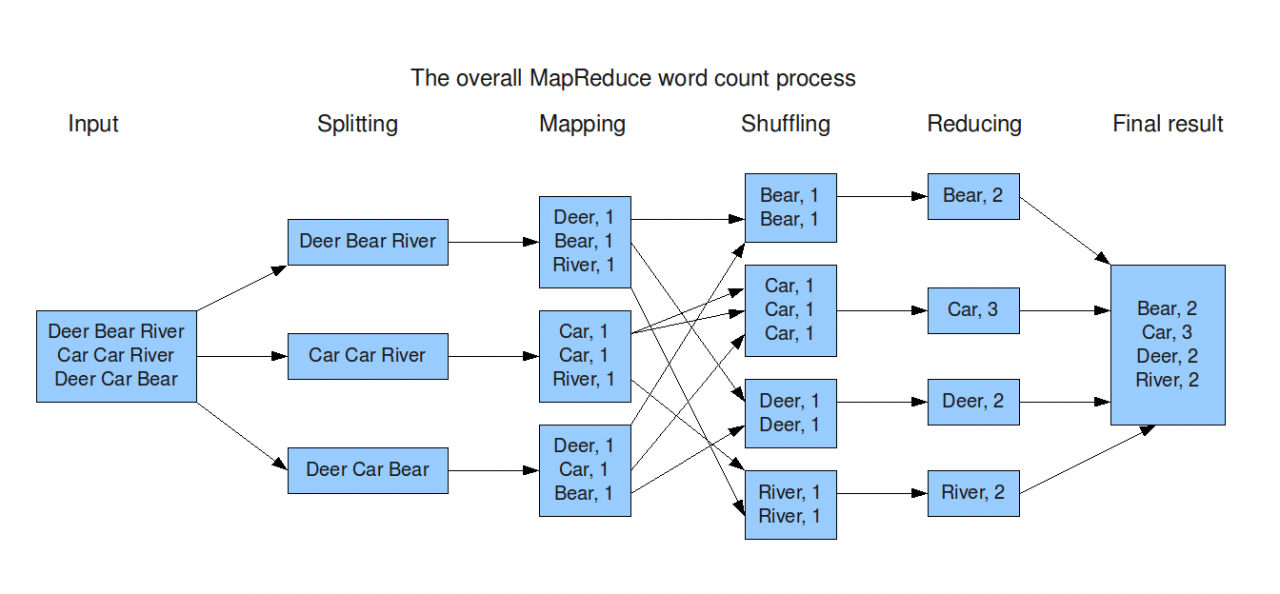
\includegraphics[width=0.8\textwidth]{figures/Wordcount.png}
      \caption{
        The Overall MapReduce Word Count Process (from http://www.learn4master.com/big-data/what-is-mapreduce-and-how-it-works)}
      \label{fig:example_figure}
    \end{center}
  \end{figure}
  \item Haddop Streaming
  Introduction: Hadoop Streaming is a generic API which allows writing Mappers and Reduces in any language. Mappers and Reducers receive their input and output on stdin and stdout as (key, value) pairs.\\
  Example: \\
  MapReduce for *nix geeks:\\
  $\#cat  data | map | sort | reduce$
  \item A Little Pig/Hive (like SQL)\\
  Differences between Pig, Hive and SQL: what we want to do in SQL is all in one long command. In Pig, we can do it in intermediate way. Hive might be quicker than SQL when doing joins. \\
  Group in Pig:\\ 
  It will give you the answer like word count in MapReduce 
  [Join (JOIN A BY a1, B BY b1)]\\
  **How we do Join in MapReduce:\\
  A(1,2,3) $\rightarrow$ [1,(A(1,2,3))]\\
  B(1,3) $\rightarrow$ [1,(B(1,2,3))]\\
  $\rightarrow$ reduce (hash join/mergesort join/…..)
\end{enumerate}


\end{document}

%%% Local Variables:
%%% mode: latex
%%% TeX-master: t
%%% End:
